\documentclass[notheorems, 9pt]{beamer}

% Packages with options
\usepackage[english]{babel}
\usepackage[mathscr]{euscript}
\usepackage[utf8]{inputenc}

% Primary Packages
\usepackage{amsbsy, amsmath, amssymb, amsthm, bm, cancel, commath, chngcntr, dsfont, econometrics, gensymb, graphicx, IEEEtrantools, longtable, marginnote, mathrsfs, mathtools, mdframed, natbib, parskip, pgf, setspace, subfigure, tabularx, textcomp, tikz}

% Rest of the setup is in the "setup_beamer" package
\usepackage{setup_beamer}

% Title, Author, Institute
\title{Econ 103: Introduction to Simple Linear Regression}
\author{Manu Navjeevan}
\institute{UCLA}

%%%%%%%%%%%%%%%%%%%%%%%%%%%%%%%%%%%%%%%%%%%%%

\begin{document}
\frame{\titlepage}
\begin{frame}{Content Outline} 
	\label{frame:content-outline}
\end{frame}
\section{The Basic Model}
\begin{frame}{Linear Regression as Line of Best Fit} 
	\label{frame:estimand}
	\onslide<+->
	Suppose we have two variables, \(Y\) and \(X\). We are interested in using data to learning about the relationship between \(Y\) and \(X\).
	
	\onslide<+->
	\red{Examples:}
	\begin{itemize}
		\item How are education and wages related?
		\item<+-> How are unemployment and inflation related?
		\item<+-> What is the relationship between receiving a treatment and a health outcome?
	\end{itemize}
	
\end{frame}
\begin{frame}{Linear Regression as Line of Best Fit} 
	\label{frame:estimand-1}
	One way to model the relationship between \(Y\) and \(X\) would be to try to find the \red{line of best fit} between the two variables. 

	By the \red{line of best fit} we mean finding the line, characterized by a slope and an intercept, that minimizes the distance between \(Y\) and \(\tilde \beta_0 + \tilde\beta_1 \cdot X\).

	\onslide<2->
	Formally, we are interested in the parameters \(\ucla{\beta_0}\) and \(\ucla{\beta_1}\) that solve
	\begin{align*}
		\ucla{\beta_0}, \ucla{\beta_1} &= \arg\min_{\tilde\beta_0,\tilde\beta_1} \E\left[\left(Y - (\tilde\beta_0 + \tilde\beta_1\cdot X)\right)^2\right] \\
									   &= \arg\min_{\tilde\beta_0,\tilde\beta_1} \E\left[\left(Y - \tilde\beta_0 -\tilde\beta_1 \cdot X\right)^2\right]
	\end{align*} 

\end{frame}
\begin{frame}{Linear Regression as Line of Best Fit} 
	\label{frame:estimand-x}
	\semitransp{One way to model the relationship between \(Y\) and \(X\) would be to try to find the line of best fit between the two variables. 

	By the line of best fit we mean finding the line, characterized by a slope and an intercept, that minimizes the distance between \(Y\) and \(\tilde \beta_0 + \tilde\beta_1 \cdot X\).

	Formally, we are interested in the parameters \(\beta_0\) and \(\beta_1\) that solve
	\begin{align*}
		\beta_0, \beta_1 &= \arg\min_{\tilde\beta_0,\tilde\beta_1} \E\left[\left(Y - (\tilde\beta_0 + \tilde\beta_1\cdot X)\right)^2\right] \\
									   &= \arg\min_{\tilde\beta_0,\tilde\beta_1} \E\left[\left(Y - \tilde\beta_0 -\tilde\beta_1 \cdot X\right)^2\right]
	\end{align*}}
	\noindent\darkucla{\rule{2cm}{0.5pt}}
	\begin{itemize}
		\item<1|only@1> By \(\arg\min\) we just mean we are interested in the \green{\bf arguments} \(\ucla{\beta_0}\) and  \(\ucla{\beta_1}\) that minimize 
		\[
				\E[(Y-\tilde\beta_0-\tilde\beta_1\cdot X)^2]
		\] 
		rather than the value \(\E[(Y-\beta_0-\beta_1\cdot X)^2]\) itself.
		\item<2|only@2> Another way of saying this is that 
		\[
			\E[(Y- \ucla{\beta_0} - \ucla{\beta_1}\cdot X)^2] < \E[(Y - \ucla{\tilde\beta_0} - \ucla{\tilde\beta_1}\cdot X)^2]
		\]
		for any \((\ucla{\tilde\beta_0},\ucla{\tilde\beta_1})\neq (\ucla{\beta_0},\ucla{\beta_1})\).
	\end{itemize}
\end{frame}
\begin{frame}{Linear Regression as Line of Best Fit} 
	\label{frame:estimand-2}
	We are interested in the parameters \(\ucla{\beta_0}\) and \(\ucla{\beta_1}\) that solve
	\begin{align*}
		\ucla{\beta_0}, \ucla{\beta_1} &= \arg\min_{\tilde\beta_0,\tilde\beta_1} \E\left[\left(Y - \tilde\beta_0 -\tilde\beta_1 \cdot X\right)^2\right]
	\end{align*}
	\red{Why do we care about these parameters?}
	\only<1>{
	\begin{itemize}
		\item<1> Knowing the line of best fit will help us predict \(Y\) using \(X\)
		\begin{itemize}
			\item<1> Will provide the \green{best linear prediction} of \(Y\) using \(X\).
			\item<1> Even though a linear model may seem to simple, ends up being tremendously useful in practice.
		\end{itemize}
	\end{itemize}}
	\only<2->{
	\begin{itemize}
	\item<2-> We can also interpret the parameters \(\beta_0\) and  \(\beta_1\) to learn (\green{to a first order degree}) about the relationship between  \(Y\) and \(X\) 
		\begin{itemize}
			\item<3-> Is there a positive or negative relationship between \(Y\) and \(X\)? \(\iff\) Is \(\beta_1\) positive or negative?
			\item<4-> How much can we expect \(Y\) to change if we see an increase in \(X\) of one unit?  \(\iff\) What is  \(\beta_1\)?
			\item<5-> What is the average value of \(Y\) when \(X\) is zero? \(\iff\) What is \(\beta_0\)?
			\item<6-> \green{To a first order degree} because \(\ucla{\beta_0}\) and \(\ucla{\beta_1}\) describe the line of best fit rather than the ``true'' relationship.
			\begin{itemize}
				\item No need to worry about this difference for now though.
			\end{itemize}
		\end{itemize}
	\end{itemize}}
\end{frame}
\begin{frame}{Linear Regression: The Parameters} 
	\label{frame:estimand-3}
	\onslide<+->
	We are interested in the parameters \(\ucla{\beta_0}\) and \(\ucla{\beta_1}\) that solve
	\begin{align*}
		\ucla{\beta_0}, \ucla{\beta_1} &= \arg\min_{\tilde\beta_0,\tilde\beta_1} \E\left[\left(Y - \tilde\beta_0 -\tilde\beta_1 \cdot X\right)^2\right]
	\end{align*}	
	\onslide<+->
	Let's solve for \(\ucla{\beta_0}\) and  \(\ucla{\beta_1}\) by taking first order conditions:
	\begin{align*}
		\frac{\partial }{\partial \tilde\beta_0}:  \E\left[Y-\ucla{\beta_0}- \ucla{\beta_1}\cdot X\right] &= 0 \\ 
		\frac{\partial }{\partial \tilde\beta_1}: \E\left[(Y-\ucla{\beta_0}-\ucla{\beta_1}\cdot X)\cdot X\right] &= 0
	\end{align*}
	\onslide<+->
	We will return to these first order conditions shortly. For now, after rearranging we get that
	\begin{align*}
		\ucla{\beta_1} &= \frac{\E[YX]-\E[Y]\E[X]}{\E[X^2]-\E[X]\E[X]} = \frac{\Cov(Y,X)}{\Var(X)}   \\
		\ucla{\beta_0} &= \E[Y] - \ucla{\beta_1}\E[X]
	\end{align*}
	\onslide<+->
	\green{Exercise: Show this rearrangement.}
\end{frame}
\begin{frame}{Linear Regression: The Error Term} 
	\label{frame:eps-1}
	Let's define the random variable
	\begin{align*}
		\eps &= Y - (\ucla{\beta_0} + \ucla{\beta_1}\cdot X) \\
			 &= Y - \ucla{\beta_0} - \ucla{\beta_1}\cdot X
	\end{align*} 
	\onslide<+->
	We can then write
	\[
		Y = \ucla{\beta_0} + \ucla{\beta_1}\cdot X + \eps
	.\] 
	which is the linear regression equation you may have seen before. The random variable \(\eps\) will be important later on as we try to do inference.
\end{frame}
\begin{frame}{Linear Regression: The Error Term} 
	\label{frame:eps-2}
	Let's define the random variable
	\begin{align*}
		\eps &= Y - (\ucla{\beta_0} + \ucla{\beta_1}\cdot X) \\
			 &= Y - \ucla{\beta_0} - \ucla{\beta_1}\cdot X
	\end{align*} 
	We call \(\eps\) the  \red{linear regression error} variable. 

	\onslide<2->
	Recall that from the first order conditions for \(\ucla{\beta_0}\) and  \(\ucla{\beta_1}\) we have that
	\begin{align*}
		\E\big[\underbrace{Y-\ucla{\beta_0}- \ucla{\beta_1}\cdot X}_{=\eps}\big] &= 0 \\ 
		\E\big[\underbrace{(Y-\ucla{\beta_0}-\ucla{\beta_1}\cdot X)}_{=\eps}\cdot X\big] &= 0
	\end{align*}
	\onslide<2->
	These give us the properties that
	\[
		\E[\eps]= 0\andbox \E[\eps X] = 0
	.\] 
\end{frame}
%TODO: Add a slide explaining how sometimes people give interpretations to error terms and it's importance to causal inference.
%TODO: Add a slide and discuss the variance of the error term as well as the conditional variance.

\begin{frame}{Linear Regression: Model Summary} 
	\label{frame:model-summary}
	In total our \red{line of best fit} parameters
	\begin{align*}
		\ucla{\beta_0}, \ucla{\beta_1} &= \arg\min_{\tilde\beta_0,\tilde\beta_1} \E\left[\left(Y - \tilde\beta_0 -\tilde\beta_1 \cdot X\right)^2\right]
	\end{align*}
	generate a model betwen \(Y\) and \(X\) that can be written as 
	\begin{equation}
		Y = \ucla{\beta_0} + \ucla{\beta_1}\cdot X + \eps
	\end{equation} 
	where 
	\[
		\E[\eps]= 0 \andbox \E[\eps X]=0
	.\]
	\onslide<2->
	\begin{itemize}
		\item It is often convenient to work directly with this representation or make assumptions about \(\eps\).
		\item You may have seen this representation before, the prior slides go over where this model comes from
	\end{itemize}
\end{frame}

\begin{frame}{Linear Regression: Model Summary} 
	\label{frame:model-summary-2}
	Our \red{line of best fit} parameters
	\begin{align*}
		\ucla{\beta_0}, \ucla{\beta_1} &= \arg\min_{\tilde\beta_0,\tilde\beta_1} \E\left[\left(Y - \tilde\beta_0 -\tilde\beta_1 \cdot X\right)^2\right]
	\end{align*}
	are useful for 
	\begin{itemize}
		\item<1-> Making predictions about \(Y\) using  \(X\).
		\begin{itemize}
			\item Predict \(Y\) when  \(X=x\) with  \(\beta_0  + \beta_1\cdot x\)
		\end{itemize}
	 \item<2-> Learning about the relationship between \(Y\) and  \(X\).
	\begin{itemize}
		\item Interpret the signs and magnitutdes of \(\beta_0\) and  \(\beta_1\)
	\end{itemize}
	\end{itemize}
\end{frame}
\begin{frame}{Linear Regression: Questions}
	\centering
	\red{\Large Questions?}
\end{frame} 

\section{Estimation}%
\label{sec:estimation}

\begin{frame}{Linear Regression: Estimation Introduction} 
	\label{frame:estimation-intro}
	As we went over in the last section we are interested in the line of best fit parameters
	\begin{align*}
		\ucla{\beta_0}, \ucla{\beta_1} &= \arg\min_{\tilde\beta_0,\tilde\beta_1} \E\left[\left(Y - \tilde\beta_0 -\tilde\beta_1 \cdot X\right)^2\right]
	\end{align*}
	\red{Problem:} We do not know know the joint distribution of \((Y,X)\), so we cannot to solve for \(\beta_0\) and  \(\beta_1\) by evaluating the expectation above. 

	\onslide<2->
	\red{Solution:} Use data to estimate the parameters \(\ucla{\beta_0}\) and  \(\ucla{\beta_1}\).
\end{frame}
\begin{frame}{Linear Regression: The Estimator} 
	\label{frame:estimator-intro}
	\red{Solution:} Use data to try and estimate the parameters \(\ucla{\beta_0}\) and  \(\ucla{\beta_1}\).

	How do we do this?
	\onslide<2->

	\ucla{Intuition:}
	\begin{itemize}
		\item<2-> Suppose we have access to \(n\) randomly collected samples  \(\{Y_i,X_i\}_{i=1}^n\)
		\item<3-> We are interested in the line of best fit between \(Y\) and \(X\) in the population
		\begin{align*}
			\ucla{\beta_0}, \ucla{\beta_1} = \arg\min_{\tilde\beta_0,\tilde\beta_1} \E\left[\left(Y - \tilde\beta_0 -\tilde\beta_1 \cdot X\right)^2\right]
		\end{align*}
		\only<4>{\item We estimate the line of best fit between \(Y\) and \(X\) in the population using the line of best fit between \(Y_i\) and \(X_i\) in our sample:
		\begin{align*}
			\ucla{\hat\beta_0},\ucla{\hat\beta_1} = \arg\min_{b_0,b_1} \frac{1}{n} \sum_{i=1}^n \left(Y_i - b_0 - b_1\cdot X_i\right)^2
		\end{align*}
		\begin{itemize}
			\item Same idea as using \(\bar X\) to estimate  \(\E[X]\), etc.
		\end{itemize}}
		\only<5>{\item We estimate the line of best fit between \(Y\) and \(X\) in the population using the line of best fit between \(Y_i\) and \(X_i\) in our sample:
		\begin{align*}
			\ucla{\hat\beta_0},\ucla{\hat\beta_1} = \arg\min_{b_0,b_1} \cancel{\frac{1}{n}} \sum_{i=1}^n \left(Y_i - b_0 - b_1\cdot X_i\right)^2
		\end{align*}
		\begin{itemize}
			\item Same idea as using \(\bar X\) to estimate  \(\E[X]\), etc.
		\end{itemize}}
	\end{itemize}
\end{frame}
\begin{frame}{Linear Regression: The Estimator} 
	\label{frame:estimator-visualization}
	Let's see how this looks like in practice. Suppose we are interested in the relationship between \(X\), a car's weight, and \(Y\) a car's miles per gallon (mpg). 

	We collect some data \(\{Y_i,X_i\}_{i=1}^n\) where each \((Y_i,X_i)\) pair represents the miles per gallon and weight of a particular vehicle in our dataset. We can represent our data using a scatterplot
	\begin{figure}[htpb]
		\centering
		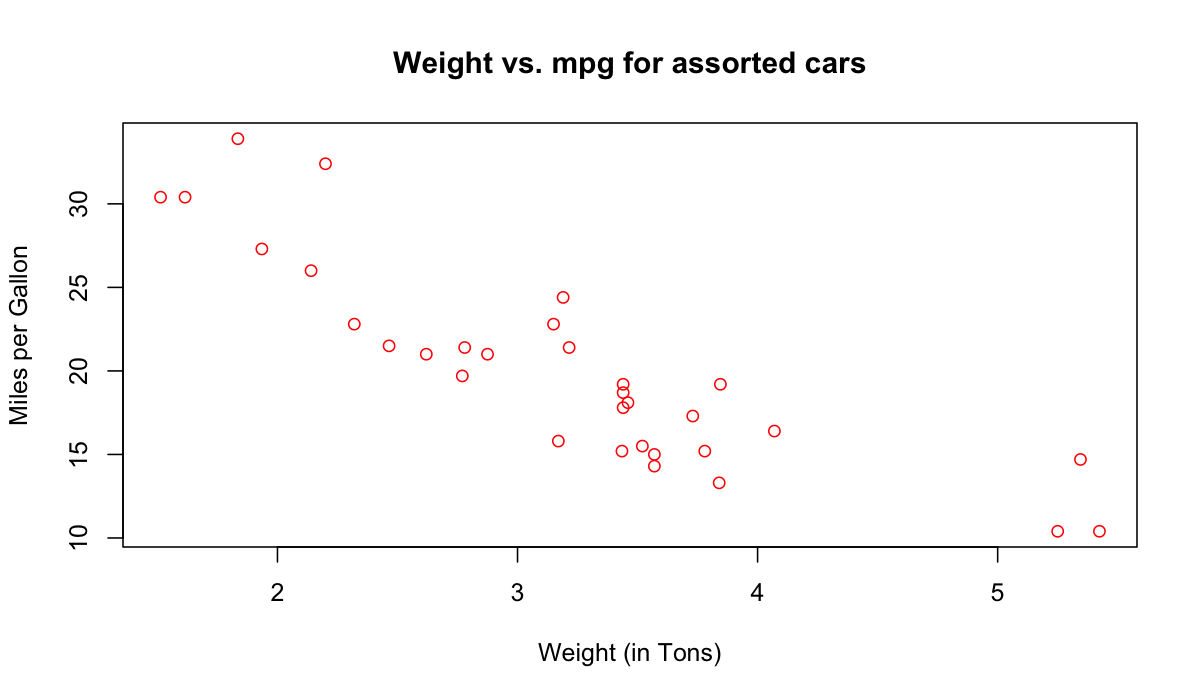
\includegraphics[width=0.8\linewidth]{scatter1.png}		
	\end{figure}
\end{frame}
\begin{frame}{Linear Regression: The Estimator} 
	\label{frame:estimator-visualization-2}
	Now to estimate \(\ucla{\hat\beta_0}, \ucla{\hat\beta_1}\) we simply find the line of best fit between the \(Y_i\) and \(X_i\) 's in our data. 
	\begin{figure}[htpb]
		\centering
		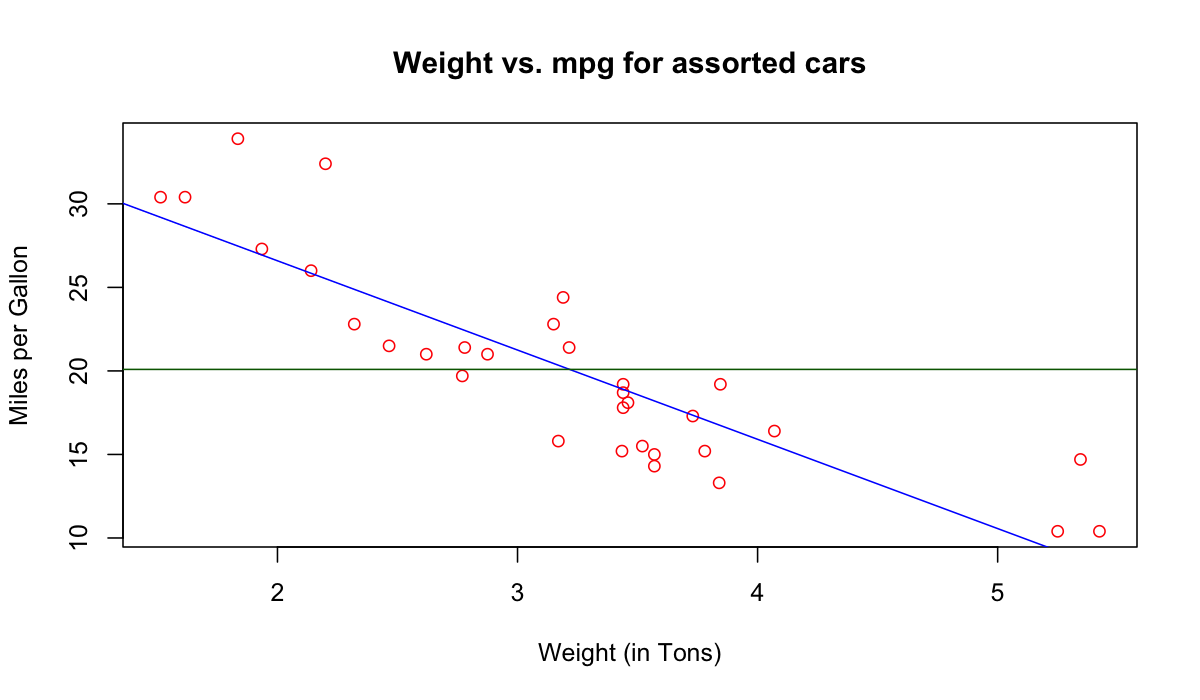
\includegraphics[width=0.8\linewidth]{scatter2.png}
	\end{figure}
	\only<2>{
	The \darkucla{blue} line represents the line of best fit whereas the \green{green} line represents a straight line through \(\bar Y\). We can see that the \darkucla{blue} line is much closer to the data than the \green{green} line.}
\end{frame}

\begin{frame}{Linear Regression: The Estimator} 
	\label{frame:estimator-2}

	In this case we have that \(\ucla{\hat\beta_0} = 37.2851\) and \(\ucla{\hat\beta_1} = -5.3445.\)

	\red{How do we interpret these estimates?}
	\begin{itemize}
		\item<2-> \(\ucla{\hat\beta_0} = 37.2851\): We estimate that the average value of  \(Y\) when  \(X=0\) is  \(37.2851\)
		\begin{itemize}
			\item In context: we estimate that the average mpg for a car that weights \(0\) tons is  \(37.2851\) miles per gallon
		\end{itemize}
		\item<3-> \(\ucla{\hat\beta_1}= -5.3445\): We estimate that, on average, a one unit increase in  \(X\) is associated with a  \(5.3445\) unit \ucla{decrease} in  \(Y\).
		\begin{itemize}
			\item In context: we estimate that, on average, a one ton increase in car weight is associated with a 5.3445 unit decrease in miles per gallon.
		\end{itemize}
	\end{itemize}
\end{frame}

\begin{frame}{Linear Regression: The Estimator} 
	\label{frame:estimator-4}
	Notice a couple things in the above interpretations
	\begin{itemize}
		\item The intercept is often uninterpretable (\green{What car would weigh 0 tons?}). For this reason we often focus our analysis on the slope coefficient. 
		\item The interpretation is deliberately not \green{causal}. We use ``associated with a decrease\dots'' as opposed to ``leads to a decrease\dots''
		%TODO: Add an explanation here for why we cannot interpret these causally
	\end{itemize} 
\end{frame}

\begin{frame}{Linear Regression: Formulas} 
	\label{frame:estimator-formula}
	Now that we've gotten some intuition for what linear regression is doing and how to use our sample to estimate the parameters of interest, let's derive explicit formulas for \(\ucla{\hat\beta_0}\) and \(\ucla{\hat\beta_1}\).

	\onslide<2->
	Recall that 
	\[
	    \ucla{\hat\beta_0},\ucla{\hat\beta_1} = \arg\min_{b_0,b_1} \frac{1}{n}\sum_{i=1}^n \left(Y_i - b_0 - b_1\cdot X_i\right)^2 
	.\] 
	\onslide<3->
	Taking first order conditions gives us that
	\begin{align*}
		\frac{\partial }{\partial b_0}: \frac{1}{n}\sum_{i=1}^n (Y_i - \ucla{\hat\beta_0} - \ucla{\hat\beta_1}\cdot X_i) &= 0 \\
		\frac{\partial }{\partial b_1}: \frac{1}{n}\sum_{i=1}^n (Y_i - \ucla{\hat\beta_0} - \ucla{\hat\beta_1}\cdot X_i)\cdot X_i &=0
	\end{align*}	
\end{frame}
\begin{frame}{Linear Regression: Formulas} 
	\label{frame:estimator-formula-1}
	Rearranging the first equality gives us
	\begin{align*}
		\frac{1}{n}\sum_{i=1}^n  Y_i - \frac{1}{n}\sum_{i=1}^n \ucla{\hat\beta_0} - \frac{1}{n}\sum_{i=1}^n \ucla{\hat\beta_1}\cdot X_i &= 0 \\
		\onslide<2->{
		\bar Y - \ucla{\hat\beta_0} - \ucla{\hat\beta_1}\frac{1}{n}\sum_{i=1}^n X_i &= 0 \\}
		\onslide<3->{
		\bar Y - \ucla{\hat\beta_0} - \ucla{\hat\beta_1}\bar X &= 0 \\
		\ucla{\hat\beta_0} &= \bar Y - \ucla{\hat\beta_1}\bar X }
	\end{align*}
	\onslide<3->
	So that what remains is to solve for \(\ucla{\hat\beta_1}\).
\end{frame}
\begin{frame}{Linear Regression: Formulas} 
	\label{frame:estimator-formula-2}
	Rearranging the second equality gives us
	\begin{align*}
		\frac{1}{n}\sum_{i=1}^n Y_i X_i - \ucla{\hat\beta_0}\frac{1}{n}\sum_{i=1}^n X_i - \ucla{\hat\beta_1}\frac{1}{n}\sum_{i=1}^n X_i^2 &= 0
		\onslide<2->{
			\intertext{Using the prior result that \( \ucla{\hat\beta_0} = \bar Y - \ucla{\hat\beta_1}\bar X\) gives:}
		\frac{1}{n}\sum_{i=1}^n Y_i X_i - (\bar Y - \ucla{\hat\beta_1}\bar X)\bar X - \ucla{\hat\beta_1}\frac{1}{n}\sum_{i=1}^n X_i^2 &= 0 \\
		\left(\frac{1}{n}\sum_{i=1}^n Y_i X_i - \bar Y \bar X\right) + \ucla{\hat\beta_1}\left((\bar X)^2 - \frac{1}{n}\sum_{i=1}^nX_i^2\right) &=0\\
		}
	\end{align*}
	\onslide<3->
	So, finally
	\[
		\ucla{\hat\beta_1} = \frac{\frac{1}{n}\sum_{i=1}^n Y_i X_i - \bar Y \bar X}{\frac{1}{n}\sum_{i=1}^n X_i^2 - (\bar X)^2} 
	.\] 
\end{frame}
\begin{frame}{Linear Regression: Formulas} 
	\label{frame:estimator-formula-3}
	Let's make use of the following equalities to represent \( \ucla{\hat\beta_1}\)
	%TODO: Assign proving these as a homework exercise
	\begin{align*}
		\frac{1}{n}\sum_{i=1}^n (Y_i - \bar Y)(X_i - \bar X) &= \frac{1}{n}\sum_{i=1}^n  Y_iX_i - \bar Y \bar X \\
		\frac{1}{n}\sum_{i=1}^n (X_i - \bar X)^2 &= \frac{1}{n}\sum_{i=1}^n X_i^2 - (\bar X)^2 
	\end{align*}
	\onslide<2->
	\red{Then:}
	\begin{align*}
		\ucla{\hat\beta_1} = \frac{\overbrace{\frac{1}{n}\sum_{i=1}^n (Y_i - \bar Y)(X_i - \bar X)}^{\text{Sample Covariance between \(Y\) and \(X\)}}}{\underbrace{\frac{1}{n}\sum_{i=1}^n (X_i - \bar X)^2 }_{\text{Sample Variance of \(X\)}}} 
	\end{align*}
	\onslide<3-> 
	This ties in nicely as, if we recall from earlier, we found that
	\[
		\ucla{\beta_1} = \frac{\Cov(Y,X)}{\Var(X)} = \frac{\E[(Y-\mu_Y)(X-\mu_X)]}{\E[(X-\mu_X)^2]} 
	.\] 
\end{frame}


\begin{frame}{Linear Regression: Randomness} 
	We have now gone over how use data to obtain estimates \(\ucla{\hat\beta_0}, \ucla{\hat\beta_1}\) of our parameters of interest \(\ucla{\beta_0}, \ucla{\beta_1}\).	
	\only<1>{
	\begin{align*}
		\ucla{\hat\beta_0},\ucla{\hat\beta_1} &= \arg\min_{b_0,b_1} \frac{1}{n}\sum_{i=1}^n \left(Y_i - b_0 - b_1\cdot X_i\right)^2 \\
		\ucla{\beta_0}, \ucla{\beta_1} &= \arg\min_{\tilde\beta_0,\tilde\beta_1} \E\left[\left(Y - \tilde\beta_0 -\tilde\beta_1 \cdot X\right)^2\right]
	\end{align*}
	}
	Notice that, while the parameters of interest \(\ucla{\beta_0}\) and  \(\ucla{\beta_1}\) are fixed quantities, the estimators \(\ucla{\hat\beta_0}\) and  \(\ucla{\hat\beta_1}\) are functions of the data; they depend on the specific sample of data collected.  
	\onslide<2->

	\red{Some Questions to Consider:}
	\begin{enumerate}
		\item<2-> What would happen to our estimates \(\ucla{\hat\beta_0}\) and \(\ucla{\hat\beta_1}\) if we were to collect a different sample of data?
		\item<3-> How can we model the distribution of our estimates \(\ucla{\hat\beta_0}\) and  \(\ucla{\hat\beta_1}\)?
		\item<4-> What happens to this distribution as \(n\to\infty\)?
	\end{enumerate}
\end{frame}
\begin{frame}{Linear Regression: Randomness} 
	\label{frame:randomness-example}
	\red{Question:} What would happen to our estimates \(\ucla{\hat\beta_0}\) and \(\ucla{\hat\beta_1}\) if we were to collect a different sample of data?

	\onslide<2->
	Let's return to the cars data and see how our regression lines look when we consider two different (random) samples.
	\begin{figure}[htpb]
		\centering
		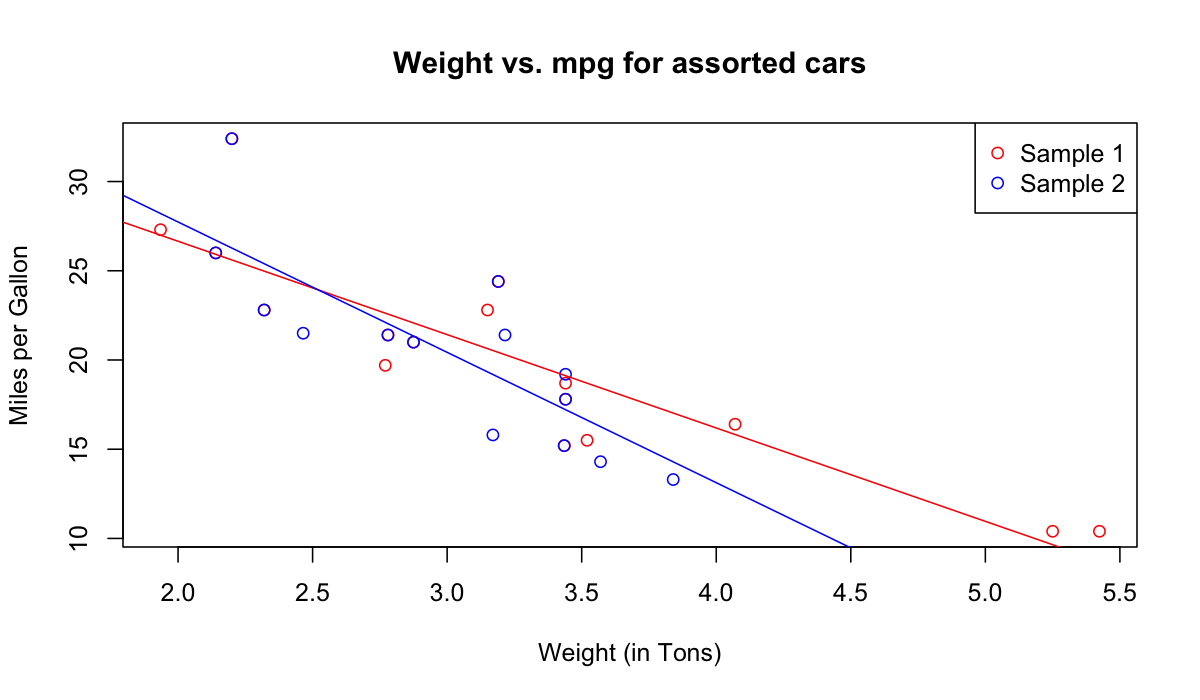
\includegraphics[width=0.75\linewidth]{scatter3.png}	
	\end{figure}
	\onslide<3->
	\begin{itemize}
		\item \red{Sample 1:} \( \ucla{\hat\beta_0} = 37.1285\) and \( \ucla{\hat\beta_1}= -5.2341\).
		\item \darkucla{Sample 2:} \( \ucla{\hat\beta_0} = 42.352\) and \( \ucla{\hat\beta_1} = -7.307\).
	\end{itemize}
\end{frame}
\begin{frame}{Linea} 
	\label{frame:}
	
\end{frame}
\section{Consistency and Inference}%
\label{sec:inference}



\end{document}


